\documentclass[]{article}

\usepackage{polski,graphicx,comment,listings,url,colortbl,tikz}
\usepackage[utf8]{inputenc}
\usepackage{algorithm}
\usepackage{algpseudocode}
\usepackage{amsmath}
\usepackage{amssymb}
\usepackage{siunitx}
\usepackage{booktabs}
\usepackage{csvsimple}

\title{Raport 4 z ECE}
\author{Paweł Ksieniewicz}

\begin{document}
\maketitle
\newpage

\section{ECE --- \emph{Exposer Classifier Ensemble}}

During the research on \textsc{ece} algorithm the development environment changed from \textsc{matlab} to \emph{Python}, which, despite the fact of obvious coding effectiveness gain, brought also a change of approach to the development process itself. Change here entails also the involuntarily change of the approach to the description of algorithm. After short introduction to the idea, this section will present a chain of development decisions leading to a final conception. Each decision will be motivated with a simple experiment showing how it affects to the classification accuracy, and each will introduce a separate element of possible \textsc{eec} configuration.

\subsection{\emph{Exposer}}
\label{exposer}

A \emph{histogram} is a \emph{graphical representation of the distribution of numerical data}. It is an estimate of the probability distribution of a continuous variable (quantitative variable) and was first introduced by Karl Pearson \cite{1895RSPTA.186..343P}. 

Construction of a histogram consist of the division\footnote{Unfortunately not the Joy Division.} of the range of values into a series of intervals, called bins and counting how many elements will fall in each of them. The bins \emph{must be adjacent} and usually are equal-sized.

A \emph{scatter plot} is a class of plot used to show distribution of two features for a set of data. The data is displayed as a cloud of points, representing objects from dataset, each corresponding with the value of chosen feature determining the position on the axes.\cite{jessica2005seeing} Example \emph{scatter plots} for \emph{iris} dataset are presented in Figure \ref{fig:scatterplots}.

A proposed data structure of \emph{exposer} is drawing from both \emph{histogram} and \emph{scatter plot}. Like in \emph{histogram}, the range of values is divided into a series of intervals, but like in a \emph{scatter plot} the combination of features is analyzed. The rule of bin adjacency is here broken, so object may fall into more than one of them. Example \emph{exposers}, generated for the same variables as the illustrated \emph{scatter plots} are presented in Figure \ref{fig:exp1}.

\begin{figure}[hbt]
	\centering
	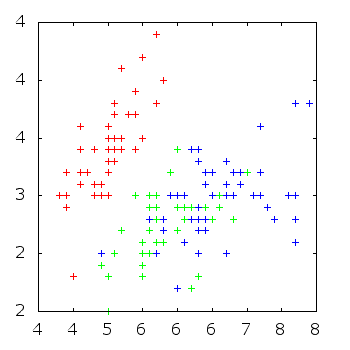
\includegraphics[width=0.32\textwidth, trim = 10 0 20 0]{figures/scatterplot_1_2}
	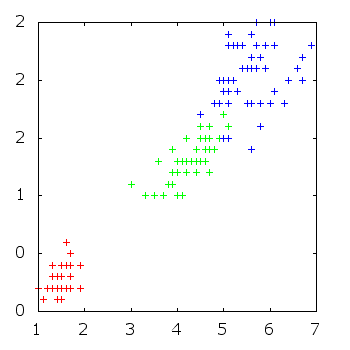
\includegraphics[width=0.32\textwidth, trim = 10 0 20 0]{figures/scatterplot_3_4}
	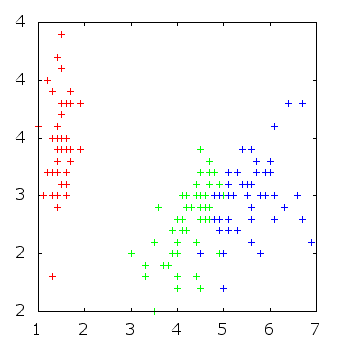
\includegraphics[width=0.32\textwidth, trim = 10 0 20 0]{figures/scatterplot_2_3}
  	\caption{Example scatter plots for \emph{iris} dataset (1:2, 3:4, 2:3)}
  	\label{fig:scatterplots}
\end{figure}

\begin{figure}[hbt]
	\centering
	
\includegraphics[width=0.305\textwidth]{figures/exponer_iris_1_2}
	
\includegraphics[width=0.305\textwidth]{figures/exponer_iris_4_3}
	
\includegraphics[width=0.305\textwidth]{figures/exponer_iris_3_2}
  	\caption{Example exposers for \emph{iris} dataset (1:2, 3:4, 2:3)}
  	\label{fig:exp1}
\end{figure}

The construction of \emph{exposer} is inspired by the process of plate light exposure of chemical photography. Hence, its control parameters are plate grain (\emph{exposer} counterpart of \emph{histograms} bin) and a light dispersion factor (called later a \emph{radius}, as a relative width of a bin according to a range of values). Instead of exposing the photographic plate coated with light-sensitive chemicals to the light source, a numerical representation matrix is exposed to the beams projected from the data samples. Procedure \emph{takes a photography} of a pair of features of the data samples, where intensity of a \emph{light} in every point is a density aggregation of the data samples falling in its neighborhood. 

The main difference from classic photography is a redefinition of the concept of color. For \emph{exposers} it consists not of classical three \textsc{rgb} spectral channels \cite{svaetichin_spectral_1956}, but of one dimension per class of the dataset. Hence, the representation matrix has as many layers as classes. The representation matrix exposure process sensitizes each layer projecting only objects from the class corresponding to the layer. There may be assumed, that \emph{exposing} procedure generates some kind of multispectral imaging \cite{1703909} from the data. 

Algorithm \ref{alg:expose} presents pseudocode used to create \emph{exposer}.

\begin{algorithm}[ht]
\caption{Expose alogorithm}
\label{alg:expose}
\begin{algorithmic}[1]
\Procedure{expose}{objects,radius,grain,features}
	\State 
	\For{$class$ \textbf{in} $classes$}
		\State $objects' \gets objects$ \emph{labeled as} $class$
		\For{$x \gets 1$ \textbf{to} $grain$}
			\For{$y \gets 1$ \textbf{to} $grain$}
				\State $base \gets (x,y) / grain$
				\State $brightness \gets 0$	
				\For{$object$ \textbf{in} $objects'$}
					\State $base' \gets object(features)$
					\State $distance \gets \sqrt{\sum{(base' -  base)^2}}$
					\If{$distance < radius$}
						\State $brightness \gets brightness (radius - distance)$
					\EndIf
				\EndFor
				\State $\mathcal{E}[x,y,class] \gets brightness$
			\EndFor
		\EndFor
	\EndFor
\EndProcedure
\end{algorithmic}
\end{algorithm}

To create a formal description, there is a set $\mathcal{X}$ of $n$ samples, $d$ features each and a set $\mathcal{M}$ of $M$ labels.

\begin{equation}
	\begin{array}[b]{llll}
		\mathcal{X} & \subseteq & \mathbb{R}^d\\
		\mathcal{M}&=&\{1, 2, \ldots, M\}\\
		x_k & = & [x_k^{(1)}, x_k^{(2)}\ldots, x_k^{(d)}],\quad x_k \in \mathcal{X}\\
		\mathcal{DS} & = & \Big\{(x_1,i_1),(x_2,i_2),\ldots,(x_n,i_n)\Big\}
	\end{array}
\end{equation}

Zdanie o tym, ze mamy zbior kombinacji $C$ z $d$ po $k$ wartościami, ktorego kazdy element $\gamma$ ma $k$ roznych od siebie wartosci.

\begin{equation}
	\begin{array}[b]{llll}
		C^k & = & \{\gamma_1^k, \ldots, \gamma_{|C^k|}^k \}\\
		\gamma_z^k & = & [x^{(t_1)}, \ldots, x^{(t_k)}], & t_1, \ldots, t_k \in \{1, \ldots, d\},\quad t_1\neq t_2 \neq \ldots \neq t_k\\
		|C^k| & = & {\;d\;\choose \;k\;}
	\end{array}
\end{equation}

A w szczegolnosci, uzywajac kombinacji dwuelementowych,

\begin{equation}
	\begin{array}[b]{llll}
		C & = & \{\gamma_1, \ldots, \gamma_{|C|} \}\\
		\gamma_z & = & [x^{(u)}, x^{(v)}], & u, v \in \{1, \ldots, d\},\quad u\neq v\\
		|C| & = & {\;d\;\choose \;2\;}
	\end{array}
\end{equation}

Representation of \emph{exposer} $E$ is an multispectral image of spatial dimensions $G\times G$ and a spectral dimension $M$, where $G$ is a \emph{grain} parameter and $M$ is a number of classes in dataset. Komentarz o dyskretyzacji.

\begin{equation}
	\begin{array}[b]{lll}
		E^k & \in & G^k \times M\\
		E^k & = & \{ E^k_1, \ldots, E^k_M \}
	\end{array}
\end{equation}

A w szczegolnosci,

\begin{equation}
	\begin{array}[b]{lll}
		E & \in & G \times G \times M\\
		E & = & \{ E_1, \ldots, E_M \}\\
	\end{array}
\end{equation}

Kazdy punkt wyznaczony przez $g_u$ i $g_v$ daje nam sygnature spektralna $pix$.

\begin{equation}
	\begin{array}[b]{lll}
		pix(g_u,g_v) &=& [pix_1(g_u,g_v), \ldots, pix_M(g_u,g_v)]
	\end{array}
\end{equation}

An entry of one layer of a \emph{exposer} ($pix_i$) is a sum of all positive differences between a given radius and a distance from a real vector of grid cell central point to the samples labeled accordingly to a layer. 

\begin{equation}
	\begin{array}[b]{lll}
		cent(pix(g_u,g_v) &=& 
	\end{array}
\end{equation}

To w zasadzie jest kwantyzacja (dyskretyzacja), na g kwantow w kazdym wymiarze przestrzennym.

\begin{equation}
	pix_i(g_u,g_v) = \sum_{k=1}^{n}\Big[d\Big(cent([g_u,g_v]),x_k\Big) < r \;\;\wedge\;\; i_k = i\Big]\;\cdot\; \Big(r - d(cent([g_u,g_v]),x_k)\Big)
\end{equation}

According to the photographic metaphor, the previous expression may be imagined as a projection by exposure, where every $x_k$ sample is the \emph{photon} with location described with features chosen by combination $\gamma$, affecting the image in $r$ radius.

Taki ekspozer pozwalalby na poprawna kolorowa wizualizacje jedynie przy trzech klasach. Aby byl uniwersalny, potrzebujemy interpretacje HSV punktu \emph{ekspozera}.

\begin{equation}
	HSV(pix) = \Big[\tfrac{argmax(pix) \times 360^\circ}{M},\;max(pix) - min(pix),\;max(pix)\Big] 
\end{equation}


\subsection{\emph{Exposer} Classifier}
\label{exposerclassifier}

Using the \emph{exposers} as a classification tool is quite easy process. There is an \emph{exposer}, exposed on a \emph{learning set} and a testing sample $x_k$ from a \emph{testing set} to classify.

\begin{equation}
	\begin{array}[b]{l}
		x_k=\{x_k^{(1)}, x_k^{(2)}, \ldots, x_k^{(d)}\},\quad\quad x_k \in \mathcal{TS}
	\end{array}
\end{equation}

Lokalizacja piksela z probki.

\begin{equation}
	fin(x) = [g_u,g_v]
\end{equation}

The prediction ($\Psi$) is the class index with the maximum value from a spectral signature $pix$ corresponding to the testing sample.

\begin{equation}
	\Psi(x_k) = \mathop{argmax}\limits_{i \in \mathcal{M}}\Bigg(pix_i\Big(fin(x_k)\Big)\Bigg)
\end{equation}

\begin{comment}

A predykcja w tym modelu ($\Psi_\textrm{\textsc{b}}$) zalezy od iloczynu wektora sygnatury z wektorem miary pewnosci.

\begin{equation}
	\Psi_\textrm{\textsc{b}}(x_k) = \textsc{argmax}\Bigg(\theta\cdot pix\Big(fin(x_k)\Big)\Bigg)
\end{equation}

	
Simple Figure \ref{fig:exp1} overwiew shows, that the classes are most discriminative with pair of features 3 and 4. How effective will be the classification of \emph{exposer} builded around them, according to a radius parameter? Intuitively a higher radius should give us an increase of accuracy.

\begin{experiment}{Radius dependency with single exposer on iris dataset.}{\small \sffamily\textbf{Description}

We are testing radius on range 0.0---0.5 using iris dataset, analyzing:

\begin{itemize}
\tightlist
	\item \texttt{2.3} --- \emph{Model}, a single exposer on lambda \textbf{[2, 3]}, grain \emph{50}, using \textbf{lone participation}.

\end{itemize}


\textbf{Results}

\centering
	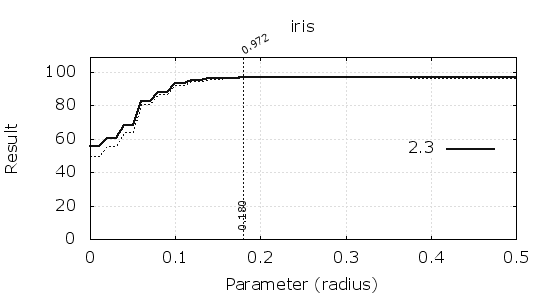
\includegraphics[width=.75\textwidth]{plots/experiment_1_iris.png}
	\captionof{figure}{Radius dependency with single exposer on iris dataset.}
	\label{fig:experiment_1}
}\end{experiment}

According to the results of Experiment 1, \emph{exposer} is a structure, which is able to be used to classify data. Hence the intuition was confirmed, it can be observed that a maximum performance of classification is achieved here quite early, with a local maximum of \verb|.18| radius. How will be the influence of \emph{grain} values onto the classification performance? Experiment 2 will try the same approach, with radius $.18$, testing grain, which intuitively should also give an increase of accuracy with highest values.
  	
\begin{experiment}{Grain dependency with single exposer on iris dataset.}{\small \sffamily\textbf{Description}

We are testing grain on range 1---40 using iris dataset, analyzing:

\begin{itemize}
\tightlist
	\item \texttt{2.3} --- \emph{Exposer one}, a single exposer on lambda \textbf{[2, 3]}, radius \emph{0.18}, using \textbf{lone participation}.

\end{itemize}


\textbf{Results}

\centering
	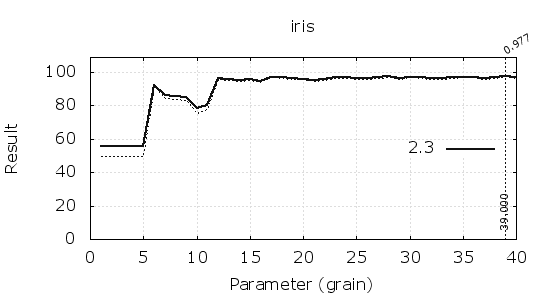
\includegraphics[width=.75\textwidth]{plots/experiment_2_iris.png}
	\captionof{figure}{Grain dependency with single exposer on iris dataset.}
	\label{fig:experiment_2}
}\end{experiment}

The similar effect of very good performance on low values of parameter was here observed. Surprisingly, the peak with the highest value of accuracy is observed here at grain set on only 15, which gave us a good performing classifier with only 225 points of data, exposed with influence of 18\%.

Figure \ref{fig:little_exposer} shows the scale of \emph{exposer}, which gave the best results for \emph{iris} dataset. $289$ Bytes of data was enough to achieve 98\% accuracy of classification.

\begin{figure}[hbt]
	\centering
	
\includegraphics[scale=1]{Figures/little_exposer}
  	\caption{Most effective \emph{exposer} on \emph{iris} dataset according to Experiments 1 and 2.}
  	\label{fig:little_exposer}
\end{figure}

\end{comment}

\subsection{\emph{Exposer} Classifier Ensemble}
\label{exposerclassifierensemble}

To establish an ensemble, a prediction procedure needs a little enhancement. There is a testing sample $x_k$ to classify.

\begin{equation}
	\begin{array}[b]{cll}
		x_k &=&\{x_k^{(1)}, x_k^{(2)}, \ldots, x_k^{(d)}\},\quad\quad x_k \in \mathcal{TS}
	\end{array}
\end{equation}

Mamy zbior \emph{ekspozerow} ($\mathcal{E}$) zbudowany na wszystkich $\gamma$ z $\Gamma$ w zbiorze uczacym oraz element zbioru testowego.

\begin{equation}
	\begin{array}[b]{cll}
		\Gamma & \subset & C,\quad\quad |\Gamma| = N,\quad\quad N \leq {d \choose k}\\
		%\mathcal{E} & = & \{E^{(1)},\ldots,E^{(N)}\}\\
		\Pi &=& \{\Psi^{(1)},\ldots,\Psi^{(N)}\}
	\end{array}
\end{equation}

Bardziej zlozony model wprowadza jednak miare pewnosci decyzji wobec kazdej z klas. Waga dla i-tej klasy to srednia saturacja ($S$) dla punktow odpowiadajacych odcieniowi klasy ($H$, $max_i(e)$) dla wartosci ($V$) większych niż zadana wielkosc graniczna. 

\begin{equation}
	\theta _i = \frac{\sum_{g_u=1}^{G}\sum_{g_v=1}^{G}\Big[ argmax(pix) = i \;\wedge\; pix_i > threshold\Big]\;S(pix)}{\sum_{g_u=1}^{G}\sum_{g_v=1}^{G} \Big[ argmax(pix) = i\Big]} 
\end{equation}

\paragraph{Voting methods}

\begin{itemize}
		\item No confidence measure
%Teraz z każdego \emph{ekspozera} ze zbioru wyliczamy wektor wsparć. Wektor wsparcia ECE to suma tych wektorów.

\begin{equation}
	\Pi_\textrm{\textsc{a}}(x_k) = \mathop{argmax}\limits_{i \in \mathcal{M}}\Bigg(\sum_{l = 1}^N pix^{(l)}\Big(fin(x_k)\Big)\Bigg)
\end{equation}

	\item Single confidence measure per class
%Teraz z każdego \emph{ekspozera} ze zbioru wyliczamy wektor wsparć. Wektor wsparcia ECE to suma tych wektorów.

\begin{equation}
	\Pi_\textrm{\textsc{b}}(x_k) = \mathop{argmax}\limits_{i \in \mathcal{M}}\Bigg(\sum_{l = 1}^N\theta^{(l)}\cdot pix^{(l)}\Big(fin(x_k)\Big)\Bigg)
\end{equation}

	\item Single confidence measure per exposer
%The linear combination of the  $\beta_i$ with $\theta_i$ weights our voting vector ($V$).

%Prediction is a class index with the maximum voting value ($\Delta$).

\begin{equation}
	\Pi_\textrm{\textsc{c}}(x_k) = \mathop{argmax}\limits_{i \in \mathcal{M}}\Bigg(\sum_{l = 1}^N mean(\theta^{(l)})\cdot pix^{(l)}\Big(fin(x_k)\Big)\Bigg)
\end{equation}

	\item Two-level confidence measure

\begin{equation}
	\Pi_\textrm{\textsc{d}}(x_k) = \mathop{argmax}\limits_{i \in \mathcal{M}}\Bigg(\sum_{l = 1}^N mean(\theta^{(l)})\cdot \theta^{(l)} \cdot pix^{(l)}\Big(fin(x_k)\Big)\Bigg)
\end{equation}

	\item Three-level confidence measure

\begin{equation}
	\Pi_\textrm{\textsc{e}}(x_k) = \mathop{argmax}\limits_{i \in \mathcal{M}}\Bigg(\sum_{l = 1}^N mean(\theta^{(l)})\cdot \theta^{(l)} \cdot pix^{(l)}\Big(fin(x_k)\Big)\cdot S\bigg(pix^{(l)}\Big(fin(x_k)\Big)\bigg)\Bigg)
\end{equation}

\end{itemize}

\paragraph{Classification model}

The classification model (Figure \ref{fig:model}) is a three-level construction. At the lowest level there is a set of monochrome layers, each of which defines a member classifier, characterized by a combination of features, denoted by $\gamma_i$, and a weight $\theta_i \in \Re^2$ used to combine its output with the remaining classifiers into \emph{exposer}. At the top level, member classifiers are combined into an \textsc{eec} ensemble.

\begin{figure*}[hbt]
	\center
  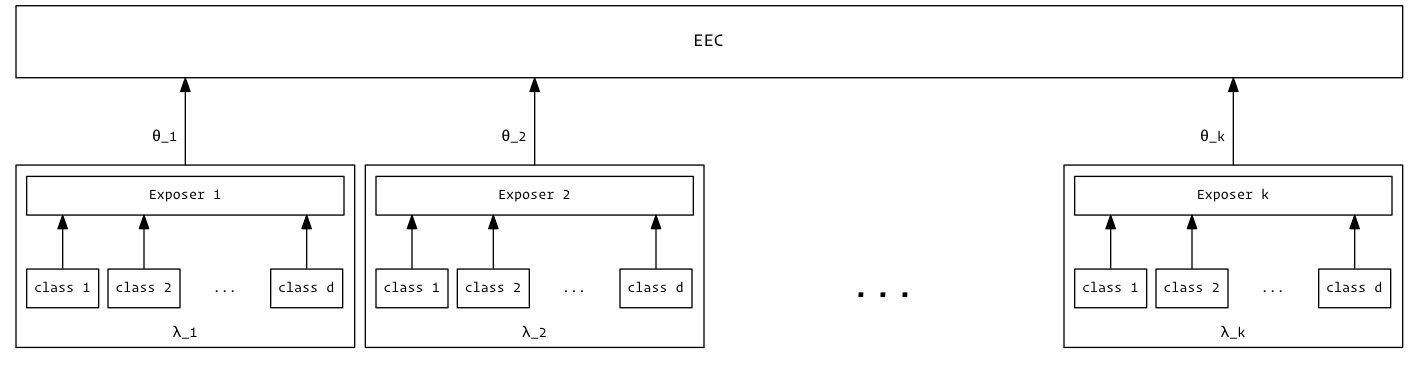
\includegraphics[width=\textwidth]{figures/eec_model}
  
  \caption{\textsc{ece} classification model diagram.}
	\label{fig:model}
\end{figure*}

\section{Ewaluacja metody}


\begin{table}[!ht]
    \sisetup{round-mode=places}
    \sisetup{
    	round-precision = 3,
    	round-integer-to-decimal
    }
    \parbox{.45\linewidth}{
		\caption{Australian}
	    \label{tab:results}
		\centering
		\begin{tabular}{lSSS}
			\toprule
			{radius} & {accuracy} & {bac} \\\midrule
		    \csvreader[head to column names]{products/australian.csv}{}%
		    {\radius & \accuracy & \bac\\}%
		\end{tabular}
	}
	\hfill
    \parbox{.45\linewidth}{
		\caption{Balance}
	    \label{tab:results}
		\centering
		\begin{tabular}{lSSS}
			\toprule
			{radius} & {accuracy} & {bac} \\\midrule
		    \csvreader[head to column names]{products/balance.csv}{}%
		    {\radius & \accuracy & \bac\\}%
		\end{tabular}
	}
\end{table}


\begin{table}[!ht]
    \sisetup{round-mode=places}
	\caption{Najlepsze accuracy}
    \label{tab:results}
    \sisetup{
    	round-precision = 3,
    	round-integer-to-decimal
    }
	\centering
	\begin{tabular}{lSSS}
		\toprule
		{dataset} & {radius} & {accuracy} \\\midrule
	    \csvreader[head to column names]{products/acc.csv}{}%
	    {\emph{\filename} & \radius & \accuracy\\}%
	\end{tabular}
\end{table}

\begin{table}[!ht]
    \sisetup{round-mode=places}
	\caption{Najlepsze bac}
    \label{tab:results}
    \sisetup{
    	round-precision = 3,
    	round-integer-to-decimal
    }
	\centering
	\begin{tabular}{lSSS}
		\toprule
		{dataset} & {radius} & {bac} \\\midrule
	    \csvreader[head to column names]{products/bac.csv}{}%
	    {\emph{\filename} & \radius & \bac\\}%
	\end{tabular}
\end{table}



\bibliographystyle{unsrt}
\bibliography{biblography}

\end{document}
